\subsection{Generating synthetic datasets} \label{meth-synth-data-subsect}
To evaluate the performance of the proposed method for clustering DNA methylation profiles a synthetic dataset is generated. 

The dataset consists of $N=400$ regions, where each region $i$ is 200bp (base pairs) long. Intuitively, location 0 may denote the Transcription Start Site (TSS), and we take 100bp (\ie locations) \emph{upstream} and 100bp \emph{downstream} of the TSS, resulting in 200bp in total. Each region $i$, may have different number of total cytosines $L_{i}$, which is randomly generated from a \emph{Binomial} distribution:
\begin{equation}
	L_{i} \sim \mathcal{B}inom(r=25, p=0.9)
\end{equation}
where $r$ is the total number of trials and $p$ is the probability of success.

Since the location of each cytosine is crucial in order to interpret the methylation profiles, these are sampled from a \emph{Uniform} distribution:
\begin{equation}
	loc_{i} \sim \mathcal{U}niform(n=L_{i}, min=-100, max=100)
\end{equation}
that is, we sample $L_{i}$ locations uniformly from (-100, 100). 

We assume that there are K=3 different methylation profiles and the clustering assignments $\mathbf{Z}$ are divided in $Z_{i}=1$ for $i \in \lbrace 1,...,200 \rbrace$, $Z_{i}=2$ for $i \in \lbrace 201,...,320 \rbrace$ and, $Z_{i}=3$ for $i \in \lbrace 321,...,400 \rbrace$. 

Finally, the observations $\mathbf{y}_{i}$ for each region $i$ are generated as follows:
\begin{itemize}
	\item{
		$Z_{i}=1$ : High methylation level upstream of TSS, followed by low methylation level downstream of TSS.
	}
	\item{ 
		$Z_{i}=2$ : Low methylation level upstream of TSS, followed by high methylation level downstream of TSS.
	}
	\item{ 
		$Z_{i}=3$ : Low methylation upstream of TSS, high methylation level around TSS, followed by low methylation level downstream of TSS.
	}
\end{itemize}

\emph{Fig. \ref{meth-prof-pic}} depicts six regions randomly selected from the synthetic dataset. Each plot represents the observations $\mathbf{y}_{i}$ for region i, and each data point represents the methylation level of the CpG in the specific location.

If someone imagines of fitting a latent function through the data points, plots (a), (b) and (c) would have similar methylation profiles, since they start with high methylation level which gradually decreases to no methylation downstream of TSS. These regions are generated from cluster $Z_{i}=1$. Plots (d) and (e) have similar methylation profiles, but very different from the other plots. These regions are generated from cluster $Z_{i}=2$. Finally, plot (f) has a distinct methylation profile with high methylation level around TSS (\ie location 0) and low methylation everywhere else and is generated from cluster $Z_{i}=3$. For clarity, each plot is coloured according to the cluster that generated it.
 
\begin{figure}[ht!]
     \begin{center}
        \subfigure[]{
            \label{fig:first1}
            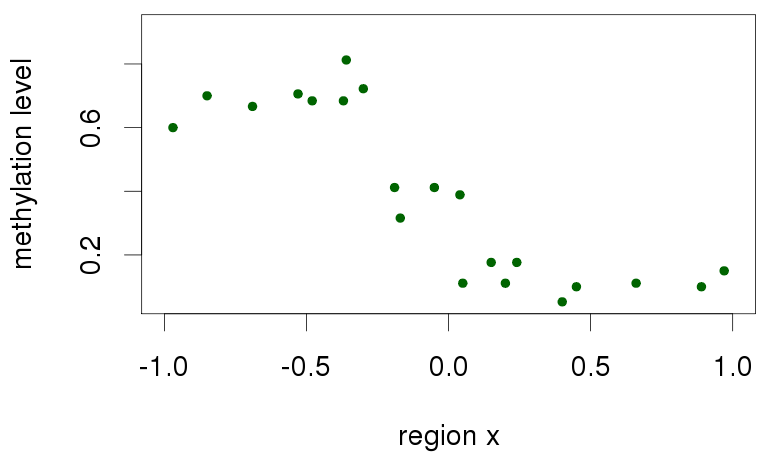
\includegraphics[width=0.31\textwidth]{images/prof1-3}
        }
        \subfigure[]{
           \label{fig:second1}
           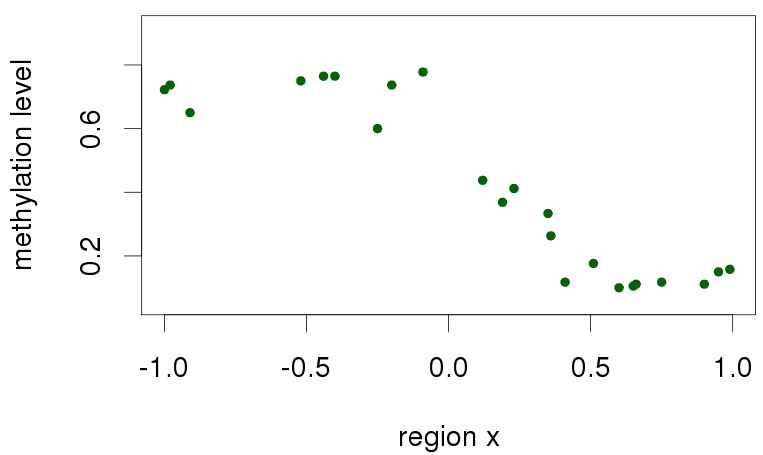
\includegraphics[width=0.31\textwidth]{images/prof2-3}
        }
        \subfigure[]{
            \label{fig:third1}
            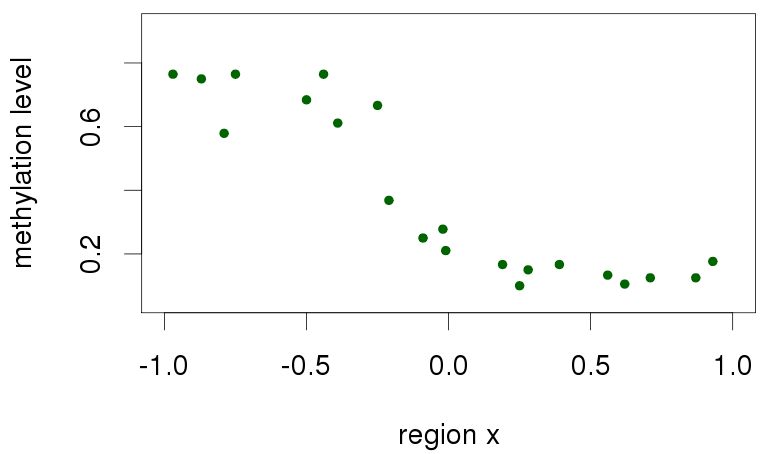
\includegraphics[width=0.31\textwidth]{images/prof3-3}
        } %  ------- End of the first row ----------------------%
        \subfigure[]{
            \label{fig:fourth1}
            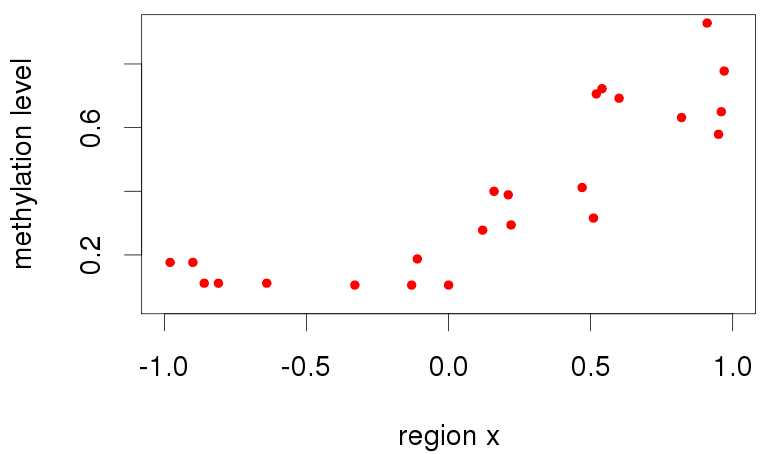
\includegraphics[width=0.31\textwidth]{images/prof4-3}
        }
        \subfigure[]{
            \label{fig:fifth1}
            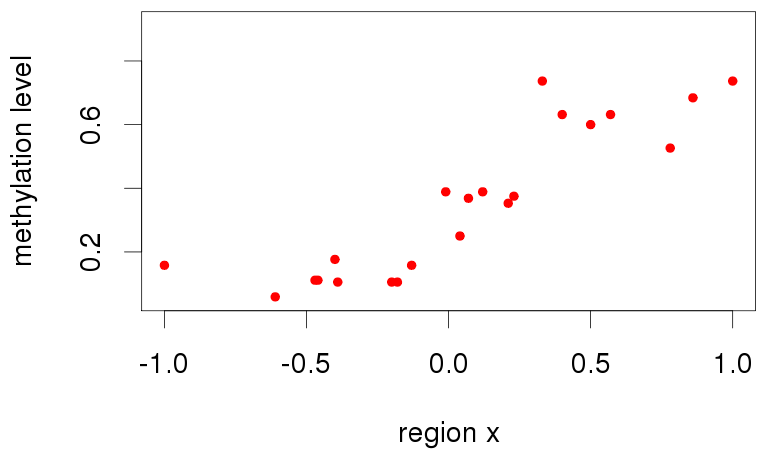
\includegraphics[width=0.31\textwidth]{images/prof5-3}
        }
        \subfigure[]{
            \label{fig:sixth1}
            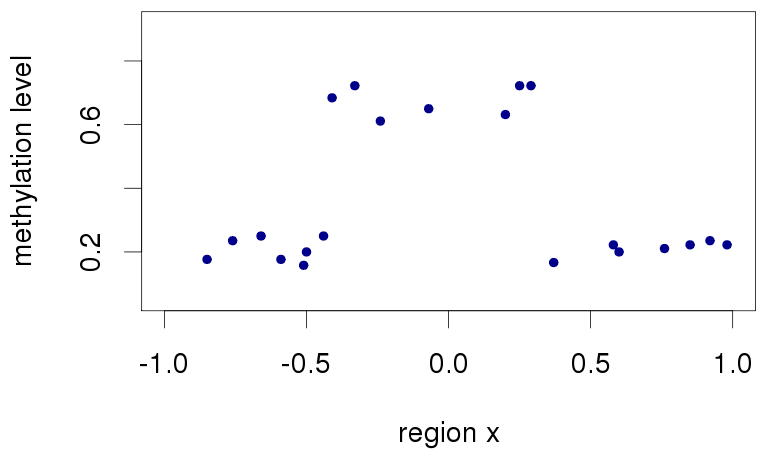
\includegraphics[width=0.31\textwidth]{images/prof6-3}
        }
    \end{center}
    \caption{\emph{Six different methylation profiles randomly chosen from the synthetic data. Each plot is coloured according to the cluster that generated it. See the text for details.}}
   \label{meth-prof-pic}
\end{figure}

It should be noted that region locations are scaled to [-1,1] interval from the [-100, 100] interval. This is mainly done for practical reasons, so as to get small values for the coefficients of the polynomials when running the EM algorithm. Location scaling was done using the following formula:
\begin{equation}
	x_{l,scaled} = \frac{x_{l} - x_{min}}{x_{max} - x_{min}} * (max - min) + min
\end{equation}
where $max=1, min=-1$, and $x_{max}$ and $x_{min}$ are the maximum and minimum values of the vector $\mathbf{x}$.